\chapter{Microscopy}
When investigating materials and specifically catalysts it is always of interest to get an impression of the three dimensional structure of the sample. This may be obtained through a strongly magnified picture of the material. Usually the conventional light microscopes are not supplying much help if we are going for the finer details such as nano-particles since their resolution is limited by the wave length of the visible light to around \SI{1}{\micro m}. Thus if want nanometer or even atomic resolution we must turn to electron microscopes and Scanning Tunnelling Microscopes (STM). We have already in connection with scanning Auger seen that a scanning electron beam can make an excellent picture of the three dimensional structure. This can be improved considerably by using several different methods for detection and by using much higher electron energies (\SIrange{200}{300}{k\electronvolt}) as it is done in dedicated electron microscopes. The ultimate resolution of electron microscopes allows a point resolution of about \SI{1}{\angstrom}, sufficient for atomic resolution. The resolution is  strongly dependent on  the nature of the sample and it is in general not surface sensitive. The main emphasis here will, however, be put on the relative new STM method. Compared to EM it is much less generally applicable, but on the other hand it offers a much more detailed view of the surface structure and dynamics, which have not been within reach before. The resolution in STM is  extremely good, less than \SI{.1}{\angstrom}, but in general it requires very flat and well defined surfaces and is therefore in reality only applicable for model systems.

\section{The Scanning Probe Methods}
The idea of scanning probe microscopes is quite simple and now exists in several versions of which the most prominent are  the STMs and Atomic Force Microscopes (AFM). The STM method was at first developed by Binning and Roher \cite{Roher1, Roher2, Roher3} (who got the Nobel prize for their invention) and this is also the most mature of the scanning probe methods (see also \cite{STM}). A sharp tip (curvature on the order of \SI{100}{\angstrom}) is brought close to a surface and a low potential difference (the bias voltage) is put between the sample and the tip. Classically there should not be a current between the sample and tip, but as the distance gets small (\SIrange{5}{10}{\angstrom}) quantum mechanics take over and the electron can now tunnel through the barrier. This leads to a current which can be measured and is typically set to be around \SI{1}{nA}. The experimental set-up is shown schematically in \autoref{fig:stmsetup}.

\begin{figure}[h!]
	\begin{center}
	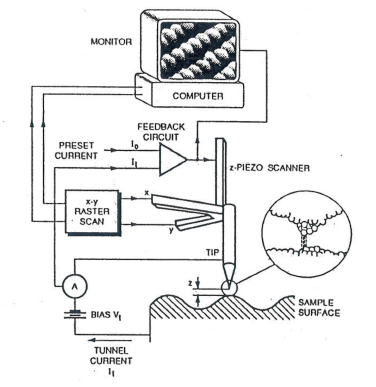
\includegraphics[scale=4]{figures/10_01.png}
	\caption{Schematics of the STM set-up.}
	\label{fig:stmsetup}
	\end{center}
\end{figure}

The experiment can be performed in several modes i.e. constant current or constant distance while scanning the tip over a desired surface area. The constant current mode is the most common. Here the current is kept constant by varying the tip-surface distance in a feedback loop. The tip is mounted on a piezoelectric tube which can expand or contract depending on the potential difference. Similarly the scanning in the $x$ and $y$ directions is obtained by applying potential differences on a tube that is split in four parts. The coarse approach of the tip to the surface is taken care of by applying a so called inch worm also based on piezoelectric elements. The scanning in the $x$ and $y$ directions goes from the \si{\angstrom} regime to a few \si{\micro m}. The inch worm allows the tip to be moved several \si{mm} per minute while the much more accurate $z$ motion is taken care of by a tube that can expand or contract typically \SI{1000}{\angstrom} with a resolution of \SI{.01}{\angstrom}! The whole arrangement is kept small to obtain high resonance frequencies and mounted on a set-up which negates external disturbances. For obtaining a typical STM picture the tip is scanning 256 lines measuring 256 points in each line. The scan rate is very fast and it takes between 1 and 10 seconds to obtain a picture. By acquiring subsequent pictures it is possible to make movies of dynamical processes on the surface such as diffusion and chemical reactions. Usually a tungsten tip is used. There are good recipes for preparing sharp tips which is necessary if the surfaces are not flat, but blunt tips prepared just by cutting a tungsten wire with pliers may also work since as long as just one atom is sticking further out than the rest this will conduct all the current as we shall see later. The disadvantage of STM is  that it unfortunately only works on reasonable well defined flat conducting surfaces.

The other scanning probe microscopy method that should be mentioned in this context is AFM. The set-up is in many ways similar to STM, although here the tip is mounted on a cantilever which is just a spring. When the tip is brought close to the surface there will be van der Waals interactions due to coulomb interactions of quantum fluctuations in the tip and substrate. This interaction sets up a potential and the tip will first feel a force when it approaches the surface. This force can be measured by measuring how much the cantilever (spring) is deflected knowing the force constant. The forces involved are extremely weak (\si{nN}) and very sensitive methods must be used to measure how much the cantilever is deflected. This is typically done by shining laser light on the cantilever which is reflected into a position sensitive detector so the motion up and down can be measured. The whole arrangement is again mounted on a piezoelectric scanner so it can be scanned over the desired area. In this manner it is possible to get atomic resolution on flat samples, or determining the  surface morphology on a larger scale. The advantage of this method is that it does not require a substrate that is conducting meaning that it can be used on real catalyst samples where the support material often is an oxide. The drawback is  that the shape of the tip, as for STM, put rather strong restrictions on the resolution and the topography that can be depicted. Like STM the method does not give any information about the composition of the surface so this information must be obtained by using complementary methods like XPS. The AFM method still undergoes strong development and may be improved considerably in the future.

In the following we will concentrate on the STM since this is the superior method and where the most interesting research is performed at the moment.

\subsection{Theory of STM}
A relatively simple and adequate theory for the tunnelling effect seen in STM was presented by Tersoff and Haman \cite{Tersoff}. Here we will only give a brief review of the involved theory and derive an expression for the essential tunnelling current. The experiment is shown schematically in \autoref{fig:stmpotential} where the energy levels of the electron in the tip and the sample are illustrated. Both are assumed to be free electron metals with monotone density of states (DOS) around the Fermi level and work function $\phi_{\mu}$  for the tip and  $\phi_{\nu}$ for the crystal. \autoref{fig:stmpotential}a illustrates the situation when the distance  between tip and surface is large. 

\begin{figure}[h!]
	\begin{center}
	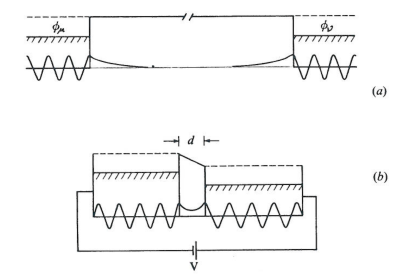
\includegraphics[scale=4]{figures/10_02.png}
	\caption{Sketch of the surface potential of the crystal and the tip.}
	\label{fig:stmpotential}
	\end{center}
\end{figure}

The  distance in \autoref{fig:stmpotential}b is now reduced to $d$ and the tip is biased negatively with a few \si{mV} with respect to the crystal. The potential for the electrons is reduced to a potential barrier with an average height of $\phi=\frac{\phi_{\mu}+\phi_{\nu}}{2}$ and as the wave functions for the electrons do not decay completely to zero they  may tunnel through the barrier. The expression for the tunnel current is in 1st order perturbation theory given by:

\begin{equation}
I=\frac{2\pi\vert e\vert}{\hbar}\sum_{\mu \nu}(f(E_{\mu})(1-F(E_{\mu})))\vert M_{\mu\nu}\vert\delta(E_{\mu}+\vert e\vert V-E_{\nu})
\end{equation}

\noindent where $E_{\mu}$ and $E_{\nu}$ are the energy relative to the Fermi level $E_F$ and

\begin{equation}
f(E)=\frac{1}{e^{\dfrac{(E-E_F)}{k_BT}}+1}
\end{equation}

\noindent is the Fermi function giving the occupation as a function of $E$. $V$ is the applied voltage difference and if $V\vert e\vert\simeq 0$ and $T \rightarrow 0$ then $f(E_{\mu}) \simeq 1$ for $E_{\mu}<0$ and $f(E_{\nu})\simeq 0$ for $E_{\nu}>0$, thus electrons are tunnelling from full states in the tip into the empty conduction states above the Fermi level of the crystal. The delta function ensures energy conservation, i.e. it is assumed that the electrons do not undergo energy losses during the mechanism. This assumption is easily seen to be fulfilled  by considering that typical bias voltages are on the order of \SI{10}{mV} and the universal curve discussed earlier. This will be truly ballistic electrons moving far into the crystal before undergoing energy losses. Using  $V\simeq 0$ and the other  approximations we get 

\begin{equation}
I=\frac{2\pi e^2V}{\hbar}\sum_{\mu\nu}\vert M_{\mu\nu}\vert\delta(E_{\mu}-E_F)\delta(E_{\nu}-E_F)
\end{equation}

The essential problem of calculating the tunnelling matrix element $M_{\mu\nu}$ was solved by Bardeen \cite{Bardeen} giving

\begin{equation}
M_{\mu\nu}=-\frac{\hbar^2}{2m}\int(\Psi_{\nu}^{\dag}\nabla\Psi_{\mu}-\Psi_{\mu} \nabla\Psi_{\nu}^{\dag})d\vec{S}
\end{equation}

Remembering that $i\hbar\nabla$ is the momentum operator it is seen that this integral evaluates the flux of electrons through a surface $S$ lying in the vacuum region.

In order to get any further we must introduce the appropriate wave functions. The wave functions at the surface of the crystal are straightforwardly described by the two-dimensional Bloch expansion as:

\begin{equation}
\Psi_{\nu}(\vec{r_{\parallel}},z)=\frac{1}{\sqrt{\Omega}}\sum_Ga_Ge^{i\vec{\kappa_G}\vec{r_{\parallel}}}e^{-z\sqrt{\kappa^2+\kappa_G^2}}
\end{equation}

\noindent where $G$ is a surface reciprocal lattice vector, $\Omega$ is a normalisation volume, and $\kappa$ is the decay constant of the surface wave into the vacuum region. $\kappa$ is given by

\begin{equation}
\kappa=\sqrt{\frac{2m\phi}{\hbar^2}}
\end{equation}

Thus the surface wave function is just an expansion on plane Bloch waves that are exponentially damped out in the vacuum region with the potential $\Phi$ as indicated in \autoref{fig:stmpotential}. The evaluation of the tip wave functions $\Psi_\mu$ is much more difficult since its structure is not known in detail. One way to approach this problem is to assume that the end of the tip can be approximated by a sphere with radius $R$ centred at position $\vec{r_0}$ as indicated in \autoref{fig:stmtip}. Then the tip waves can be approximated by s-waves of the type

\begin{equation}
\psi_{\mu}=\frac{1}{\sqrt{\Omega_t}}c_t \kappa Re^{\kappa R}\frac{e^{-\kappa\vert r-r_0\vert}}{\kappa\vert r-r_0\vert}
\end{equation}
 
\noindent where $\Omega_t$ is the normalisation volume and $c_t$ is a normalisation constant.

\begin{figure}[h!]
	\begin{center}
	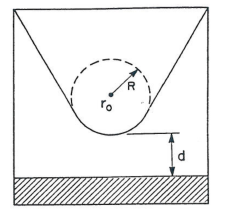
\includegraphics[scale=4]{figures/10_03.png}
	\caption{Model of the tip close to the surface.}
	\label{fig:stmtip}
	\end{center}
\end{figure}

The matrix element can now be calculated leading to

\begin{equation}
M_{\nu\mu}=\frac{1}{\sqrt{\Omega_t}}\frac{4\pi\hbar^2}{2m}Re^{\kappa R}\Psi_{\nu}(\vec{r_0})
\end{equation}

\noindent inserting this in the equation for the current $I$ we get

\begin{equation}
I=\frac{8\pi\hbar^3e^2R^2V}{m}e^{\kappa R}D_t(E_F)\rho(\vec{r_0},E_f)
\end{equation}

\noindent where $D_t=\frac{1}{\Omega_t}\sum_{\mu}\delta(E_{\mu}-E)$ is the density of states per volume of the tip and

\begin{equation}
\rho(\vec{r},E_f)=\sum_{\nu}\vert\Psi_{\mu} \vert^2\delta(E_{\nu}-E)
\end{equation}

\noindent is the local density of states at the crystal. The surface wave functions are exponentially damped out in vacuum where there is a mean potential $\Phi$ resulting in

\begin{equation}
 \vert\Psi_{\mu}\vert^2\propto e^{-2\kappa z}
\end{equation}

\noindent leading to the final equation

\begin{equation}
I\propto e^{-2\kappa z}=e^{-1.025\sqrt{\Phi(\si{\electronvolt})}z(\si{\angstrom})}
\end{equation}

The main result is that the current is exponentially dependent on the distance between the tip and the surface, mainly because the overlap between the empty and filled wave is dependent on the tails of the wave function out in the vacuum region. This explains why it is not extremely difficult to get a good and localised tip. Consider one atom on the tip that sticks out with just \SI{1}{\angstrom} compared to the rest, then it will carry \SI{90}{\percent} of the current. This also explains why it is possible to obtain atomic resolution in STM. Finally it should be mentioned that for  fixed tip conditions we will probe the density of states (either empty if the tip is negatively biased or filled states if the tip is positively biased) of the crystal just below the tip. Thus what is depicted in an STM experiment is {\bf not} the atoms but the density of states around the Fermi level. That this density varies around the atoms leading to the observed corrugation is not a surprise.

The above model involved many approximations and assumptions, nevertheless, it captures the most important features of the STM experiment. Naturally there are regions where this picture will break down due to its simplicity. If for example the tip surface distance is getting very small the potential barrier will not be a simple average any longer and eventually there will be formed a contact. This contact can consist of a single atom and it is then seen how the conductance becomes quantised. This is an interesting phenomenon but beyond the scope of these notes. Also if the current is getting very high this simple picture will break down since we have completely neglected the interaction between the tunnelling electrons. Thus care must be exercised.

\subsection{Results from the Yellium Model}
In order to elucidate how adsorbates will be depicted in STM N. Lang \cite{Lang} undertook a number of investigations using  a simple model system. The tip was modelled by a Na atom adsorbed on a high electron density metal which can be described by the so called yellium model. Here the positive charge from the nuclei are smeared out and the free electron gas is solved on this positive background. One advantage of such models is that it is relatively easy to map out the difference in eigenstate density introduced by adding an adsorbate to the yellium. \autoref{fig:esdensity} shows such differences when Mo, Na and S is adsorbed on a yellium. The calculation is only shown for $m=0$ component of the wavefunctions since it is these states that are mainly  responsible for  the tunnelling current. The figure shows that Na introduces a resonance above the Fermi level while S introduces one below and all three components result in additional charge density at the Fermi level.

Using this set-up and positioning the "tip" i.e. the yellium with an adsorbed  Na atom in front of another yellium it was shown that the current density was indeed localised to the Na atom as shown in \autoref{fig:idensity}. The largest current density arrow is a factor of 25 bigger than the smallest current density $j_0$. The length and the thickness of the current arrows are proportional to $1+ln(j/j_0)$.

\begin{figure}[h!]
	\begin{center}
	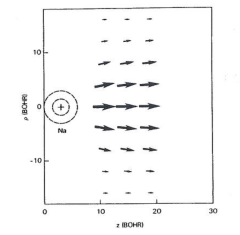
\includegraphics[scale=4.2]{figures/10_04.png}
	\caption{Difference in eigenstate density between the yellium-adsorbate system and the clean yellium for different adsorbates as indicated, taken from \cite{Lang}.}
	\label{fig:esdensity}
	\end{center}
\end{figure}

\begin{figure}[h!]
	\begin{center}
	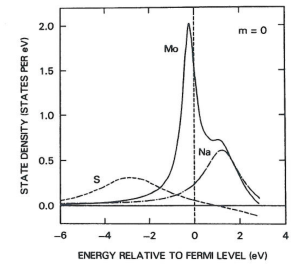
\includegraphics[scale=4]{figures/10_05.png}
	\caption{Current density for a "tip" consisting of a Na atom adsorbed on a yellium positioned in front of a clean yellium surface. The length and thickness of the arrows are proportional to $1+\ln(j/j_0)$. Taken from \cite{Lang}.}
	\label{fig:idensity}
	\end{center}
\end{figure}

If this "tip" is now used to scan over another yellium where adsorbates like Na, S and He have been adsorbed it is possible to estimate how much the tip have to be displaced vertically in order to keep the current constant when a small bias voltage is applied. This is depicted in \autoref{fig:tipdisplacement} showing that Na will appear as a much larger protrusion than S while He will be depicted as a depression in the yellium. This is in good agreement with \autoref{fig:esdensity} showing that Na introduces a much higher electron density at the Fermi level than  S does and since the tunnelling current was proportional to the density of states at the Fermi level it will lead to a larger retraction of the tip in the Na case. The He will naturally not adsorb at all, but will, due to the Pauli principle, exclude the electron leading to a lowering of density of states with respect to the clean surface.

\begin{figure}[h!]
	\begin{center}
	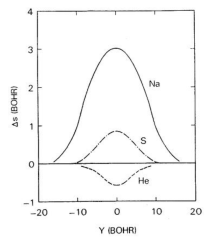
\includegraphics[scale=4]{figures/10_06.png}
	\caption{Displacement of the "tip" in the  constant current mode for Na, S, and He adsorbed on yellium, taken from \cite{Lang}.}
	\label{fig:tipdisplacement}
	\end{center}
\end{figure}

The important thing to be learned from this, is that adsorbates may not necessarily be depicted as protrusions, although they are geometrically. It all depends on the effective charge density at the Fermi level and it is well known that adsorbates like carbon, nitrogen, and  oxygen all are depicted as holes, since they are relatively electronegative and removes charge density from the Fermi level. This also shows that we must know what sort of adsorbates we are dealing with i.e. the experiment must be conducted under well defined conditions.

\section{Spectroscopy}
In all the considerations above the bias voltage was kept low so only the states around the Fermi level participated in the tunnelling phenomenon. If we now changed this condition and used higher potentials $V$ the tunnelling current will be dependent on the density of states at higher energy levels, making it possible to map out the DOS below and above the Fermi level doing spectroscopy. The current can be approximated by

\begin{equation}
I\propto\int_{E_F}^{E_F+\vert e\vert V}\rho_{\nu}(\vec{r_0},E)\rho_{\mu}(E-\dim e\dim V)dE
\end{equation}

\noindent where $\rho_{\mu}$ is the total density of states of the tip and $\rho_{\nu}$ is the local density of the sample. The $\rho_{\nu}$ can  be approximated by a product of the density at the surface times a penetration factor out into the forbidden vacuum region as:

\begin{equation}
\rho_{\nu}(\vec{r_0},E)\sim\rho_{\nu}(E)e^{-\dfrac{2d\sqrt{2m(W-E+\dfrac{1}{2})\vert e\vert V}}{\hbar}}
\end{equation}

\noindent where $W$ is the height of the potential barrier. This is intuitively easy to understand. The lower the energy $E$ the broader and higher the barrier will be and the current will therefore be dampened exponentially. If we want to isolate $\rho_{\nu}(E)$ we must clean it from the influence of the penetration factor and $\rho_{\mu}$ . By measuring relations between $I$ and $V$ for a fixed distance and by plotting  $(dI/dV)/(I/V)$ any sharp feature in the surface (or tip) density of states will become apparent. An example was given by Lang shown in \autoref{fig:dos} where the Na "tip" was used on a Ca atom adsorbed on yellium. The left panel shows the difference in density of states for the two adsorbates and the left panel shows the resulting $(dI/dV)/(I/V)$ analysis. Only broad features are in general observed for metals so this method is, like UPS, useless for elemental analysis.

\begin{figure}[h!]
	\begin{center}
	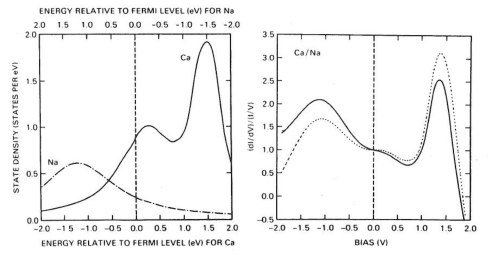
\includegraphics[scale=4.2]{figures/10_07.png}
	\caption{Left: The introduced difference in density of states by adsorbing Na and Ca on yellium. Right: The resulting $(dI/dV)/(I/V)$ analysis, taken from \cite{Lang}.}
	\label{fig:dos}
	\end{center}
\end{figure}

It is worth noticing that if we look at S adsorbed on the yellium we see that the appearance in an STM experiment will depend very much on the bias potential, since it, as shown in \autoref{fig:dosanddisplacement}, leads to a reduced density of states at high voltages. Thus, as indicated in \autoref{fig:dosanddisplacement}, the S atom will appear as a protrusion for voltages below \SI{1}{V}, will vanish around \SI{1.3}{V} and become a depression for higher voltages. Thus the picture obtainable will be very dependent on the chosen bias voltage. This is in particular illustrated in semiconductors where there is a bandgap and dangling bond pairs to form occupied bonding states and empty anti bonding states at the surface. By making $(dI/dV)/(I/V)$ analysis the various states can be found for a constant distance and by scanning  at well chosen voltages the different orbitals can be mapped out on the surface.

\begin{figure}[h!]
	\begin{center}
	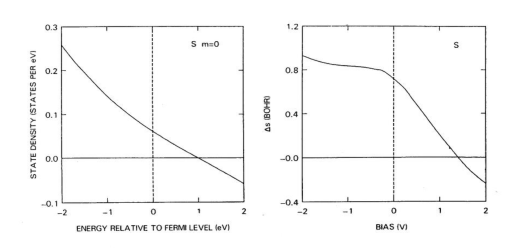
\includegraphics[scale=4.2]{figures/10_08.png}
	\caption{Left: The introduced difference in density of states by adsorbing Na and S on yellium. Right: The vertical displacement of the "tip" over the S atom as a function of bias voltage, taken from \cite{Lang}.}
	\label{fig:dosanddisplacement}
	\end{center}
\end{figure}

In the above we have assumed that the tip behaves like a metal. Not much is in reality known for sure about the states of the tip and the ad atom actually conducting the current. Sometimes the tip changes in the middle of a scan and what earlier appeared as protrusions may suddenly in the middle of a frame be  depicted as depressions or vice versa. Such sudden and unexplained changes are often interpreted as tip changes, where the tip for example is picking up an atom  from the surface changing its nature.

\section{Examples of STM Investigations}
STM has had a very strong impact on the field of surface science and STM have to some extent also revolutionised the structural investigation. Still, it is not a trivial method to use like LEED where it is possible to obtain a LEED pattern within than half an hour if the surface is well ordered. It can be somewhat tricky to prepare the tip so that high resolution pictures can be  obtained. Sometimes, the STM  is working immediately, other times one may spend a day at the microscope and only occasionally see a structure. It is particularly difficult to obtain atomic resolution on metal surfaces since the corrugation here usually is less than \SI{0.1}{\angstrom}.

The STM and LEED methods complement each other in the sense that LEED rather quickly gives an idea of the overall order on the surface, but not much information on the atomic level if that is not ordered. Luckily STM works very well at this level. In principle STM does not require any order on the surface meaning that domain boundaries and positions of single atoms can be investigated in great detail. So in principle the STM is much more versatile, although it should be remembered that just because we see an interesting structure within an area of $100\times 100 \si{\angstrom^2}$, it is not necessarily representative for the rest of the surface. Therefore several areas must  be investigated before any conclusions can be drawn. In the following we will give a few examples on the use of STM.

\subsection{Surface Structure}
Acquiring an STM picture of a surface structure actually provides us with a real space picture of the surface topography, although care should be exercised, since it is the electron density at the Fermi level we are mapping out. Atoms that sticks out from the surface may  not necessarily become depicted as protrusions. Usually it is possible to recognise the unit cell although that does not provide a solution to the structure. An example is shown in \autoref{fig:stmleed} where the STM pictures and the LEED pattern of the S-Cu(100) $(\sqrt{17}\times\sqrt{17})R\ang{14}$ is shown.

Although it is known from AES studies that this surface contains eight sulphur atoms per unit cell only four of them can be identified as protrusions in the STM picture. The corresponding LEED pattern is quite complex as there are two domains. A model based on the STM picture have been proposed and is shown in \autoref{fig:scumodel}.

\begin{figure}[h!]
	\begin{center}
	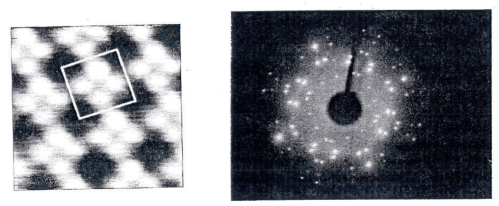
\includegraphics[scale=4]{figures/10_09.png}
	\caption{STM and LEED picture of the S-Cu(100) $(\sqrt{17} \times \sqrt{17})$R\ang{14} structure, taken from \cite{Luigi}.}
	\label{fig:stmleed}
	\end{center}
\end{figure}

\begin{figure}[h!]
	\begin{center}
	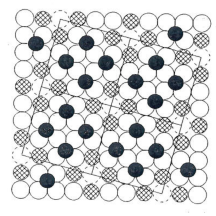
\includegraphics[scale=4]{figures/10_10.png}
	\caption{A schematic model of the S-Cu(100) $(\sqrt{17} \times \sqrt{17})$R\ang{14} structure with eight sulphur atoms per unit cell, taken from \cite{Luigi}.}
	\label{fig:scumodel}
	\end{center}
\end{figure}

Sometimes it is possible to observe both regions of the clean metal and regions covered with an adsorbate so it is possible to extend the metal lattice into the adsorbate structure. This is demonstrated in \autoref{fig:ocustm} taken from Besenbacher \textit{et al}. \cite{Besenbacher1} where the STM picture of the Cu(110) and the missing O-Cu(110) $(2\times 1)$ row are shown.

\begin{figure}[h!]
	\begin{center}
	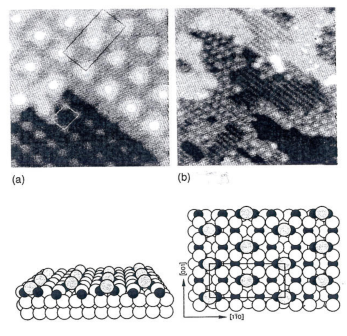
\includegraphics[scale=4]{figures/10_11.png}
	\caption{STM picture showing the coexistence of the O-Cu(110)($2\times 1$) and the O-Cu(110)c($6\times 2$) structures on a Cu(110) c($6Ztimes 2$) structure on a Cu(110) surface. a) $51\times \SI{50}{\angstrom^2}$ and b) $157\times \SI{171}{\angstrom^2}$. c) and d) show models of the O-Cu(110)c($6\times 2$) structure from the side and topview, respectively. The oxygen atoms are depicted as black, while the copper atoms are depicted as gray or white.}
	\label{fig:ocustm}
	\end{center}
\end{figure}

Also by detailed analysis of the surface as a function of adsorbate dose it is possible to estimate how much of the substrate is being build into a new structure by following the mass transport of the substrate, i.e. following the  development of steps and holes made in the crystal as a function of dose. By making movies of the oxidation of Cu(110) it was for example possible to suggest a structure for the high coverage structure O-Cu(110) c$(6\times 2)$ which, quite surprisingly, showed that Cu atoms were sitting highly uncoordinated on top of the previously formed missing row reconstructions as shown in \autoref{fig:ocustm2} \cite{Besenbacher1}. A structure where the unit cell is very difficult to solve in the conventional LEED-IV analysis.

\begin{figure}[h!]
	\begin{center}
	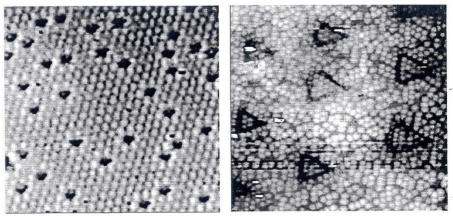
\includegraphics[scale=4]{figures/10_12.png}
	\caption{Atomically resolved STM pictures of Au deposited on Ni(111) at elevated temperature. The Au atoms are depicted as depressions. The left picture shows an area of $51\times \SI{49}{\angstrom^2}$ with a coverage of \SI{0.3}{ML} showing that the Au atoms alloy into the surface. At coverages beyond \SI{0.3}{ML} (picture to the right, $109\times \SI{109}{\angstrom^2}$) both the surface alloy and the superstructure consisting of triangular misfit dislocations are seen.}
	\label{fig:ocustm2}
	\end{center}
\end{figure}

\subsection{Two-Dimensional Alloys and Overlayers}
Since there is no help to be found from spectroscopic analysis for distinguishing two metals from each other it can be a difficult task to investigate metal overlayers and alloy formations. But again if the development of the surface can be followed as a function of deposition time, changes can be related to the amount of metal added. It is in this manner possible to study growth and diffusion mechanisms even on homo epitaxial systems like Pt deposited on a Pt single crystal. Earlier, the  growth mechanisms on surfaces were classified into  three modes as  mentioned  in Chapter \ref{ch:auger} (Frank-van der Merwe, Stranski-Krastanov and Volmer-Weber growth modes). However, the STM have shown that that was a much too simplified picture and that there is many other complex ways the growth process may proceed. Also alloy formation can be investigated and it was recently shown by use of STM that even metals which are known to be immiscible can form two-dimensional alloys in the surface. It has now been found to be a quite common phenomenon \cite{Besenbacher2} and we shall here describe  one of the first systems that was found.

If Au is deposited on Ni(111) it was expected that the Au would grow epitaxially on the Ni surface because the system was known to be immiscible and the surface energy of Au is significantly smaller than Ni. Thus it was surprising when STM pictures, like the one shown in \autoref{fig:cocostm}, were measured \cite{Besenbacher3}. Since the coverage of the black holes increased with increasing Au dose these were identified as being due to gold. At the same time some very bright atoms also appeared and it turned out to be Ni atoms pressed out from the surface by the gold. Thus a two-dimensional nearly random surface alloy was being formed in this case. Actually the Au atoms have been calculated to protrude by about a quarter of an \si{\angstrom} from the Ni surface, but again due to the electron density around the Fermi level  they appear like depressions in the Ni lattice. This two-dimensional surface structure proved to be a very good way to control the  reactivity of Ni particles and a catalyst was later developed on that basis \cite{Science}.

\begin{figure}[h!]
	\begin{center}
	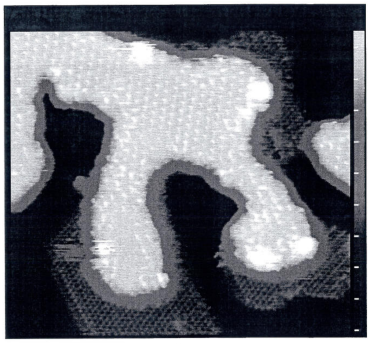
\includegraphics[scale=4]{figures/10_13.png}
	\caption{The STM picture ($140\times \SI{160}{\angstrom^2}$) shows a two layer high Co surrounded by a Cu brim. That the central part of the island consisted of Co was determined by exposing the surface to CO at room temperature where CO only adsorbs on Co leading to the observed($\sqrt{3}\times\sqrt{3}$)structure of CO on Co.}
	\label{fig:cocostm}
	\end{center}
\end{figure}

The Co-Cu(111) system is an example of studying overlayers on the surface. Again the structures that was found when depositing Co at room temperature were not simple islands in the submonolayer regime. Instead, two layer high islands were found surrounded by a single layer high island. By adsorbing CO it was possible to identify,  that the central island consisted of Co while the surrounding island consisted of Cu. An STM picture of CO on Co/Cu(111) at room temperature is shown in \autoref{fig:cucosketch} taken from \cite{Morten}. CO was only adsorbed on Co sites at this temperature, and the $(\sqrt{3}\times\sqrt{3})R\ang{30}$ of CO on Co can be recognized in the top layer \cite{Morten}. Around the apparent double layered Co island there is a Cu brim which with time will become double layered at room temperature. 

\begin{figure}[h!]
	\begin{center}
	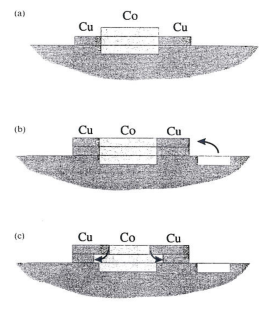
\includegraphics[scale=4]{figures/10_14.png}
	\caption{Sketch of the formation of three layer high Co islands. The surrounding Cu brim is pressed out by the Co island even when depositing the Co at low temperature (\SI{170}{K}). By heating the sample slightly the Cu brim also grows two layer thick and eventually the whole Co island will be covered by Cu.}
	\label{fig:cucosketch}
	\end{center}
\end{figure}

Based on such STM pictures with atomic resolution, a model was proposed which is schematically illustrated in \autoref{fig:emscheme}. Thus co-adsorption of for example CO made it possible to distinguish the Co from Cu. It should in this context be mentioned that it is usually very difficult to obtain pictures of CO adsorbed on surfaces, since this species diffuse very fast compared to the time scale of the STM experiment. Only in the saturation coverage regime the CO structure will freeze out and pictures like the one shown in \autoref{fig:cucosketch} are  obtainable.

\begin{figure}[h!]
	\begin{center}
	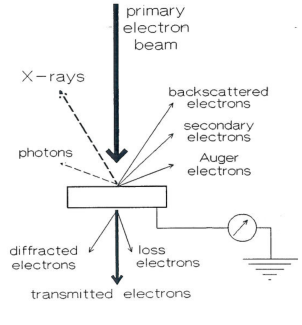
\includegraphics[scale=4]{figures/10_15.png}
	\caption{The Electron Microscope shown schematically with the various detection possibilities \cite{Niemantsverdriet}.}
	\label{fig:emscheme}
	\end{center}
\end{figure}

\subsection{Dynamics and Chemical Reactions}
By acquiring sequences of pictures it is possible to follow the dynamics on the surface if the processes are taking place on the same time scale as the measurements. This is mainly a matter of being able to control the temperature of the sample while scanning. Unfortunately, that is not a trivial problem, since the sample must be isolated from vibrations and any temperature difference may lead to thermal drift in the system. Nevertheless, there is a strong development in the field and there have recently been many studies both below and above room temperature. 

Diffusion of ad atoms or adsorbates can for example be studied and by following their two-dimensional movement the diffusion constant can be extracted. Also regular chemical reactions may be followed. One example is the oxidation of methanol on the O-Cu(110) ($2\times 1$) structure where it has been shown that the reaction is very anisotropic and only takes place at the rim of the oxygen islands. This implies that at that particular temperature the mean field approximation is not valid. Such experiments require long time stability of the STM and surprisingly few good investigations have actually been performed. This is also an area of development, since there is a strong demand for being able to run the STM not only at elevated temperatures but also at elevated pressures from the catalysis community. Any STM can run under ambient conditions, but the challenge is to get it running in atmospheres relevant to catalysis and study reactions at the surface. There have been attempts to obtain STM images of real catalysts, but so far it has not been very successful. It is very difficult to orient yourself on such non-ideal surfaces and find the active metal particles. Furthermore there is also the problem of the isolating the support material.

\section{Electron Microscopy}
Electron Microscopy is widely used giving us a visual impression of materials or biological samples in the regime where the light microscopes does not work any longer. Considering  the universal curve  it is obvious that these \SIrange{100}{400}{k\electronvolt} electrons will penetrate their way into the sample and the method is as such not a surface sensitive method, although it can be if combined with for example an Auger analyser. There are many ways to detect the electrons used in EM as shown in \autoref{fig:rhsitem} taken from \cite{Niemantsverdriet} and each of the methods add complementary information on the sample investigated. 

\begin{figure}[h!]
 	\begin{center}
 	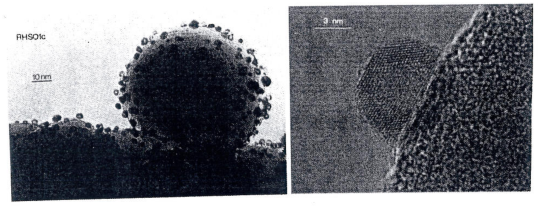
\includegraphics[scale=4]{figures/10_16.png}
 	\caption{Transmission Electron Micrograph of Rh particles dispersed on a silica sphere.}
 	\label{fig:rhsitem}
 	\end{center}
\end{figure} 

The transmitted (TEM) or reflected (SEM) electrons may in the scanning mode be used for depicting the sample morphology. By measuring emitted x-rays (EDX), emitted electrons (Auger), or by measuring energy losses it is possible to make elemental identifications. The electrons may undergo diffraction, if there are favourably oriented crystalline particles so also crystallographic information may be obtained. An example  of a transmission electron micrograph, stimulating our imagination of a catalyst, is shown in \autoref{fig:cnisio2tem} where small Rh particles are supported on a silica sphere \cite{Datye}.

\begin{figure}[h!]
	\begin{center}
	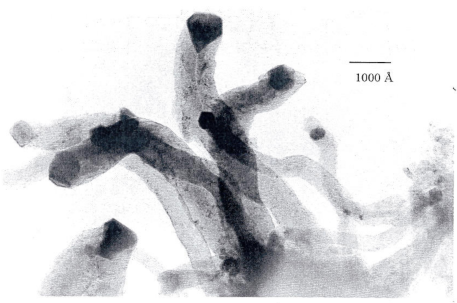
\includegraphics[scale=4]{figures/10_17.png}
	\caption{Transmission electron microscope picture of the carbon formation and filament growth on a \ce{SiO2} supported Ni catalyst after exposure to a \ce{CH4} and \ce{H2} mixture at \SI{1}{bar} and \SI{763}{K}. The dark pear shaped areas are the Ni particles which are approximately \SI{1000}{\angstrom} in diameter. The carbon is believed to have diffused through the Ni particles, forming long carbon filaments between the Ni particle and the support material.}
	\label{fig:cnisio2tem}
	\end{center}
\end{figure}

Another example is the highly undesired growth of carbon on Ni-catalyst as shown in \autoref{fig:cnistm}. Here it is seen how the carbon filaments grow out from the Ni-particles basically ruining the catalyst, taken from \cite{carbon}.

\begin{figure}[h!]
	\begin{center}
	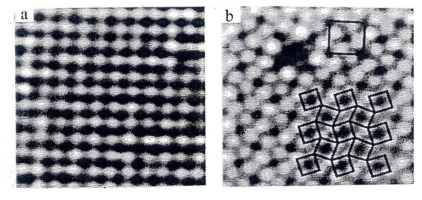
\includegraphics[scale=4]{figures/10_18.png}
	\caption{STM picture of clean Ni(100) and the carbon induced clock reconstruction on Ni(100). A model is also included.}
	\label{fig:cnistm}
	\end{center}
\end{figure}

EM microscopes usually come in the conventional high vacuum regime (\SIrange{e-6}{e-7}{mbar}) or in the UHV version (\SI{e-10}{mbar}). But  recent development have made it possible to study samples under reasonable pressures (mbar regime) so catalysts can be studied under somewhat more realistic conditions following for example the dynamics as a function of gas composition. Care must naturally be taken here since an \SI{300}{k\electronvolt} beam is not exactly innocent concerning introducing chemical reactions, that would not otherwise have been possible.

\section{Problems}
\begin{enumerate}
\item We have shown that the tunnel current $I$ is proportional to $\exp((-4\pi z\sqrt{2m\phi})/h)$, where $m$ is the mass of an electron, $\phi$ is the barrier height(work function), and $h$ is Planck's constant. Calculate the relative change in tunnelling current if the distance between tip and surface is changed \SI{1}{\angstrom}.

\item In an STM experiment the bias voltage is set to \SI{0.010}{V} and the requested tunnelling current to \SI{2.0}{nA}. Estimate the current density if we assume that all the electrons are tunnelling from only one atom at the tip (is this a realistic assumption?). Can the tunnelling process be considered as a one electron process? Discuss the size of the deposited power per volume. Can that have any influence on the measurements performed? It should for completeness be mentioned that it has been found that the STM tip can be used both to introduce chemical reactions on the surface and for manipulating atoms. This has perspectives for reaching the ultimate level of data storage.

\item \autoref{fig:cnistm} is an STM picture of clean Ni(100) and the reconstructed Ni(100)-($2\times 2$)p4g-C and the model. What does the respective LEED patterns look like?

\item Assume we have a well ordered surface (why?). Will the Fourier transform of the STM picture always be identical to the LEED pattern?
\end{enumerate}